\section{Simulation Analysis}
\label{sec:simulation}

In this section, Ngspice was used in order to simulate the audio converter, therefore, a brief description of the circuit modeled in NGspice is going to be presented and a comparison between the values obtained in NGspice and the ones in Octave is going to be done as well. In order to do that, transistors of the given models were used and the rest of the components specifications changed to be on par with the values through MatLab.


\subsection{Coupling Capacitor}




\subsection{Bypass Capacitor}





\subsection{$R_c$}





\subsection{Comparison}





%\begin{table}[H] \centering
%\begin{tabular}{|
%>{\columncolor[HTML]{FFCC67}}l |c|}
%\hline
%\multicolumn{2}{|l|}{\cellcolor[HTML]{EABD8B}Name - Value} \\ \hline
%Cost & 2619.6\\ \hline
merit & 1262.83\\ \hline

%\end{tabular}
%\caption{COST}
%\end{table}

%\begin{table}[H] \centering
%\begin{tabular}{|
%>{\columncolor[HTML]{FFCC67}}l |c|}
%\hline
%\multicolumn{2}{|l|}{\cellcolor[HTML]{EABD8B}Name - Value} \\ \hline
%V_CE&4.71217\\ \hline
V_BE&0.642988\\ \hline
V_CE>V_BE & Correct F.A.R\\ \hline

%\end{tabular}
%\caption{NPN}
%\end{table}

%\begin{table}[H] \centering
%\begin{tabular}{|
%>{\columncolor[HTML]{FFCC67}}l |c|}
%\hline
%\multicolumn{2}{|l|}{\cellcolor[HTML]{EABD8B}Name - Value} \\ \hline
%V_CE&6.83806\\ \hline
V_EB&0.785099\\ \hline
V_EC>V_EB & Correct F.A.R\\ \hline

%\end{tabular}
%\caption{PNP}
%\end{table}

%\begin{table}[H] \centering
%\begin{tabular}{|
%>{\columncolor[HTML]{FFCC67}}l |c|}
%\hline
%\multicolumn{2}{|l|}{\cellcolor[HTML]{EABD8B}Name - Value} \\ \hline
%V-Gain & 34.1988\\ \hline
Bandwidth & 1.22501E+06\\ \hline
CO-lowerFreq & 15.8734\\ \hline
CO-higherFreq & 1.22503E+06\\ \hline

%\end{tabular}
%\caption{Results for the output}
%\end{table}

%\begin{table}[H] \centering
%\begin{tabular}{|
%>{\columncolor[HTML]{FFCC67}}l |c|}
%\hline
%\multicolumn{2}{|l|}{\cellcolor[HTML]{EABD8B}Name - Value} \\ \hline
%Zin & 999.002 + -7.3282 j\\ \hline

%\end{tabular}
%\caption{Results for the output of the envelope}
%\end{table}

\begin{figure}[H] 
\centering
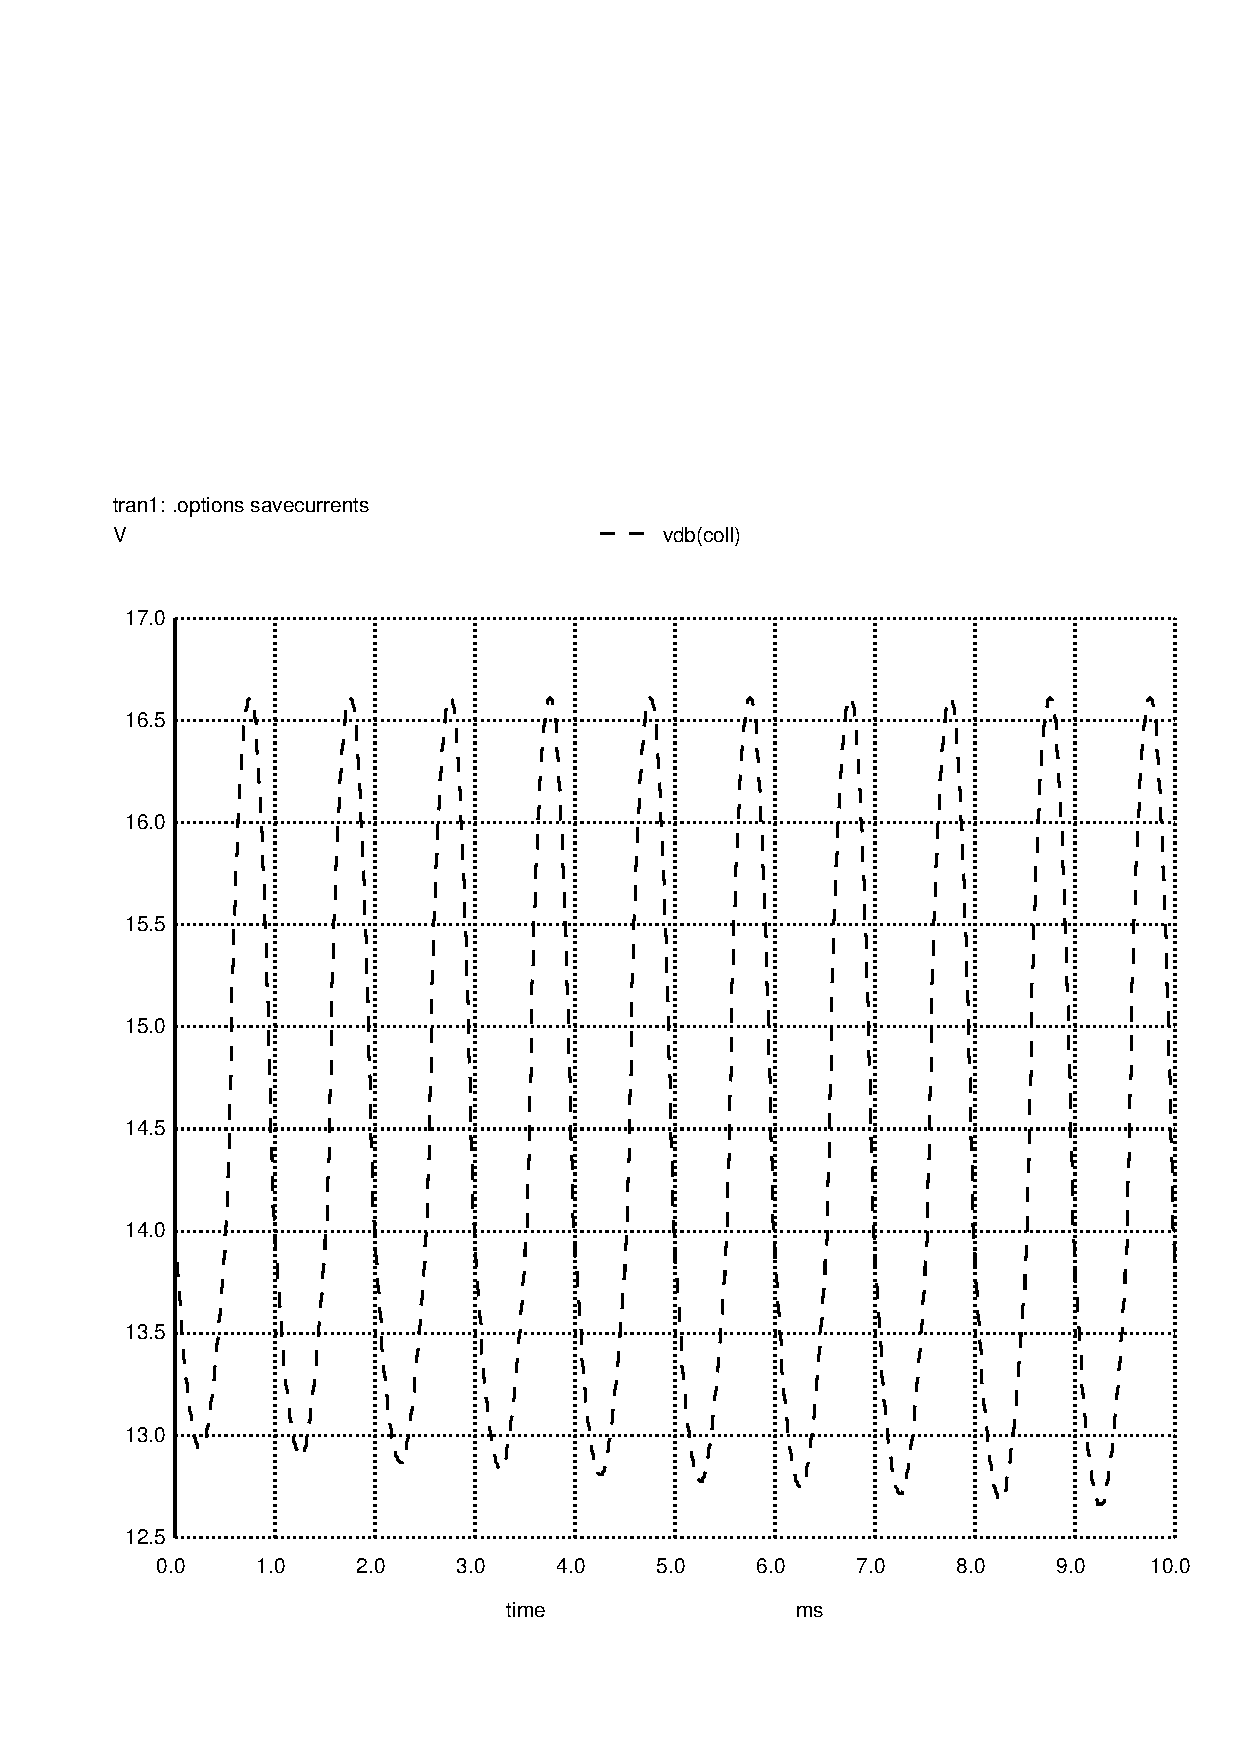
\includegraphics[width = 8cm]{vo1.pdf} 
\caption{Output}
\label{vo1}
\end{figure}

\begin{figure}[H] 
\centering
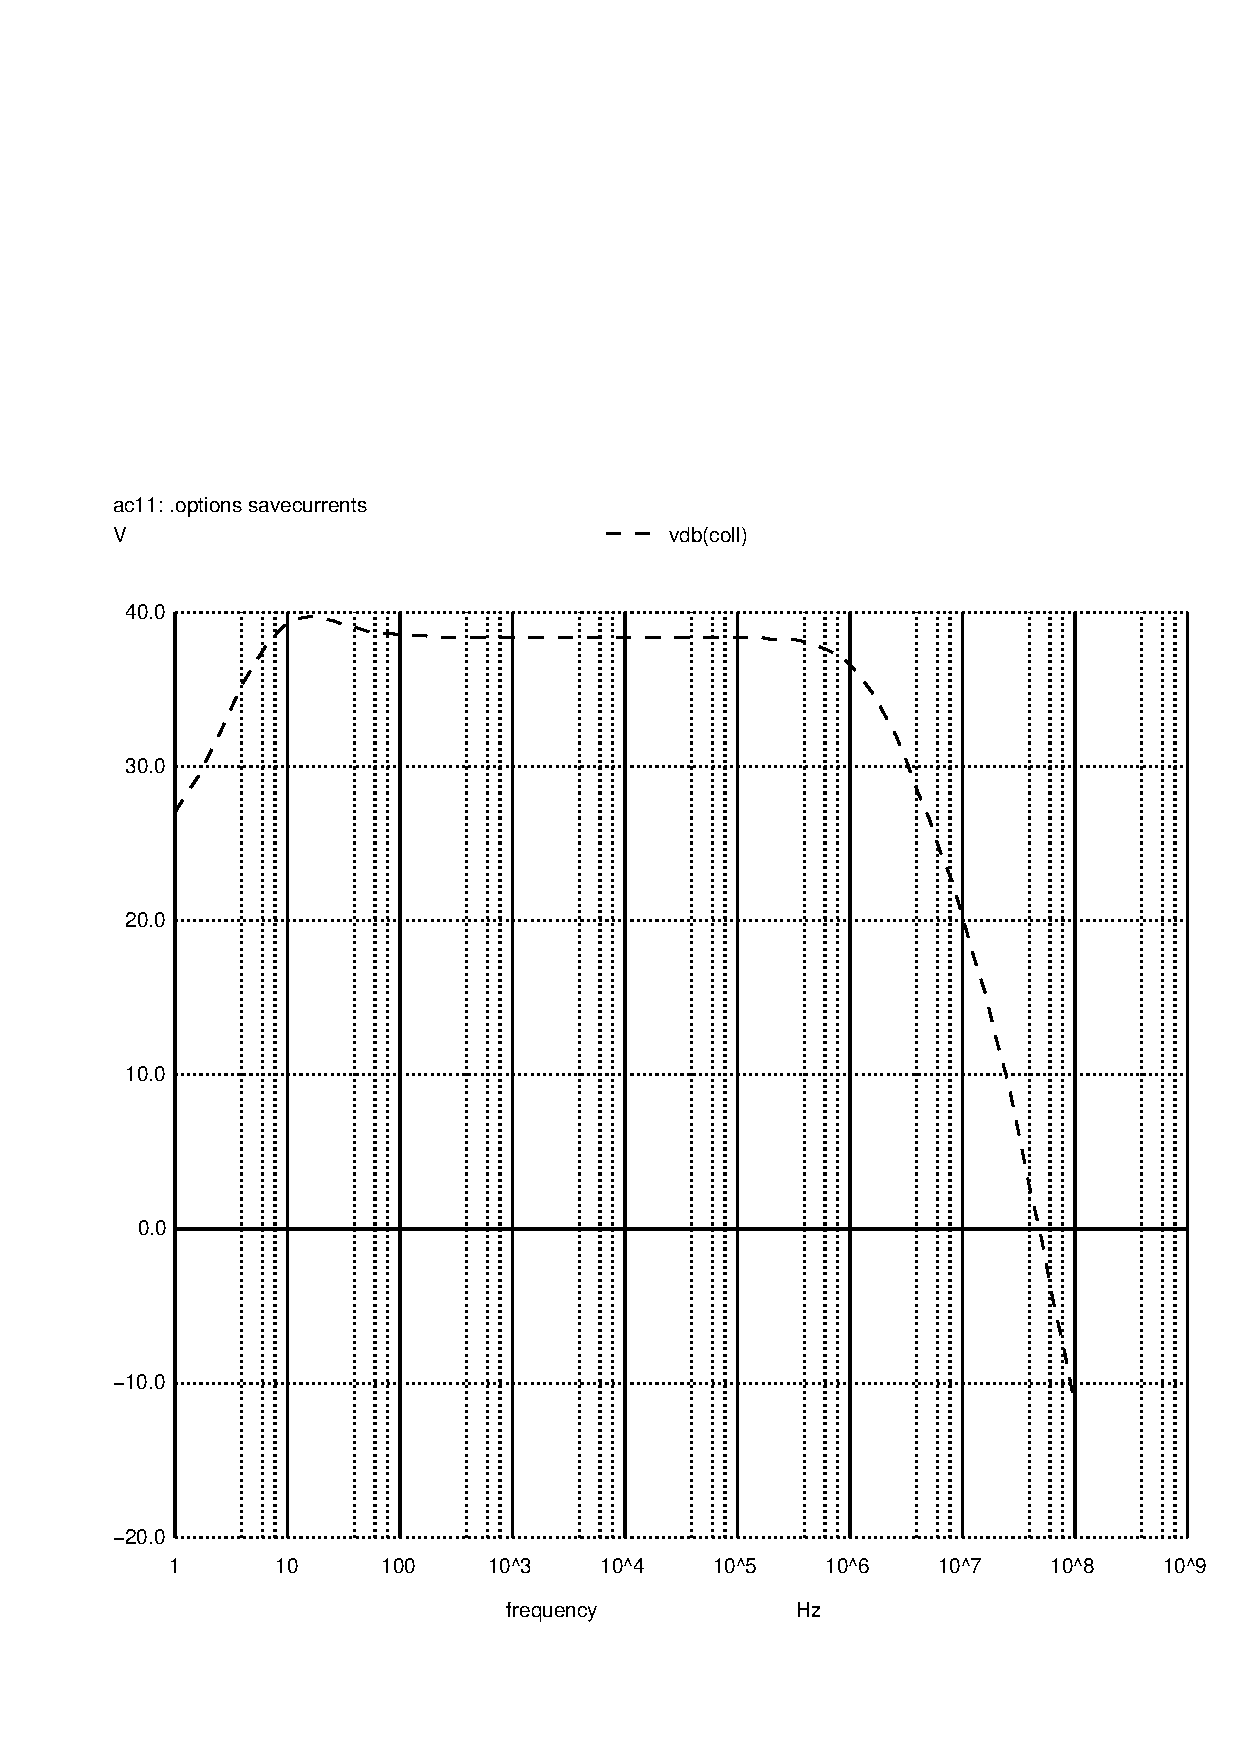
\includegraphics[width = 8cm]{vo1f.pdf} 
\caption{Output}
\label{vo1f}
\end{figure}

\begin{figure}[H] 
\centering
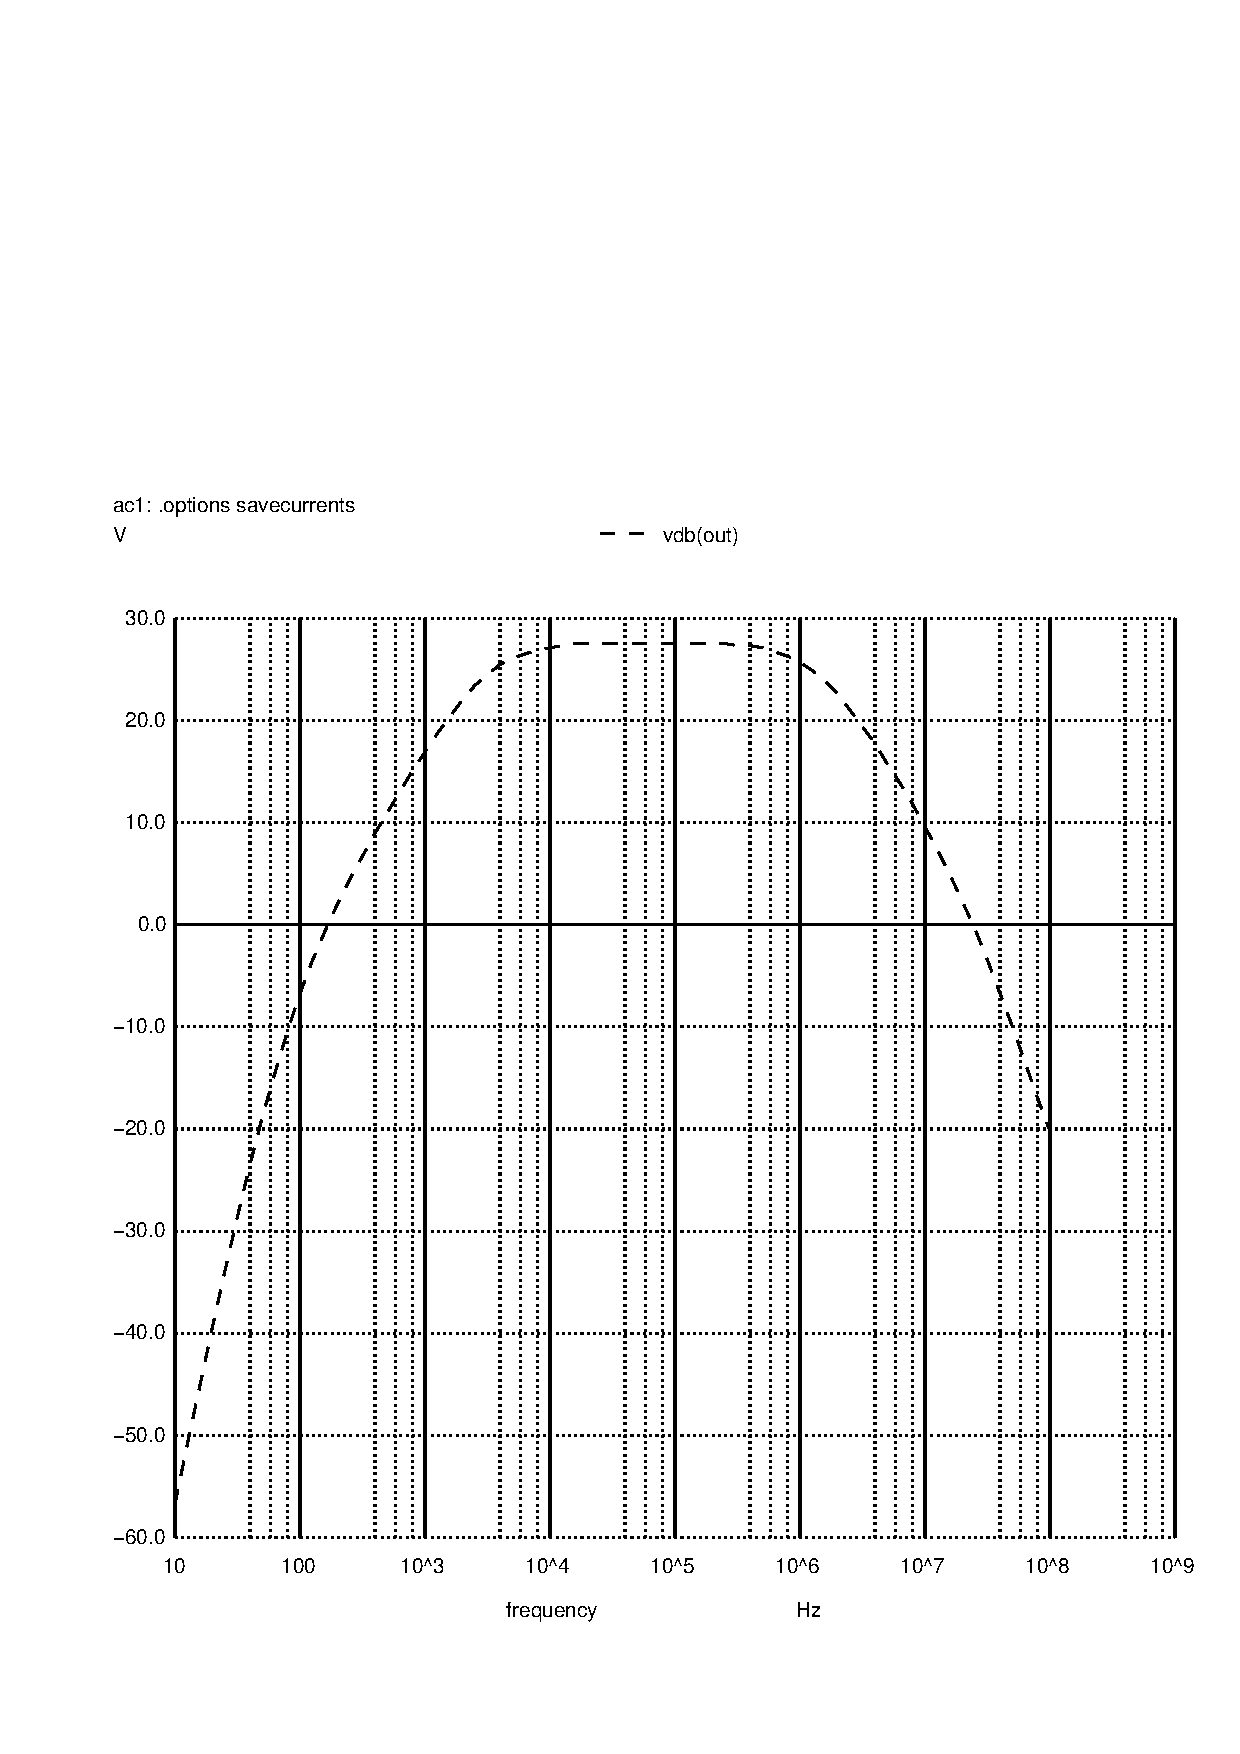
\includegraphics[width = 8cm]{vo2f.pdf} 
\caption{Output}
\label{vo2f}
\end{figure}

\subsection{Merit Results}

From the results obtained through the Ngspice simulation and considering we used the data shown in table 1, we can compute the merit using the formula given in the lab assignment, represented in the Introduction.

The implemented circuit gave us a MERIT of ??? in NGSpice.



